% !TEX root=report.tex
\section{CouchSurfing Experience and Data} \label{sec:data}

CouchSurfing.org is a worldwide network that envisions ``a world where everyone can explore and create meaningful connections with the people and places they encounter.''\footnote{Retrieved from http://www.couchsurfing.org/about.html/vision}
More than four million users participate in the site through hosting travelers on their own couch, ``surfing'' on other users' couches when traveling in a foreign city, or finding and participating in local CouchSurfing meetups in their area \cite{Lauterbach2009}. CouchSurfers have been to 252 different countries and speak 366 unique languages.\footnote{Retrieved from http://www.couchsurfing.org/statistics.html}
Being a part of a social travel community, each user presents themselves in their user profile (see Figure \ref{fig:csprofile} for an example). These profiles contain rich information about the user, their CouchSurfing experience, what languages they speak, their interest, which countries they have traveled to, and much more.
\todo{We could include some stats about our dataset here (i.e. the still relevant parts in Data Exploration)}

\begin{figure}[ht]
\centering
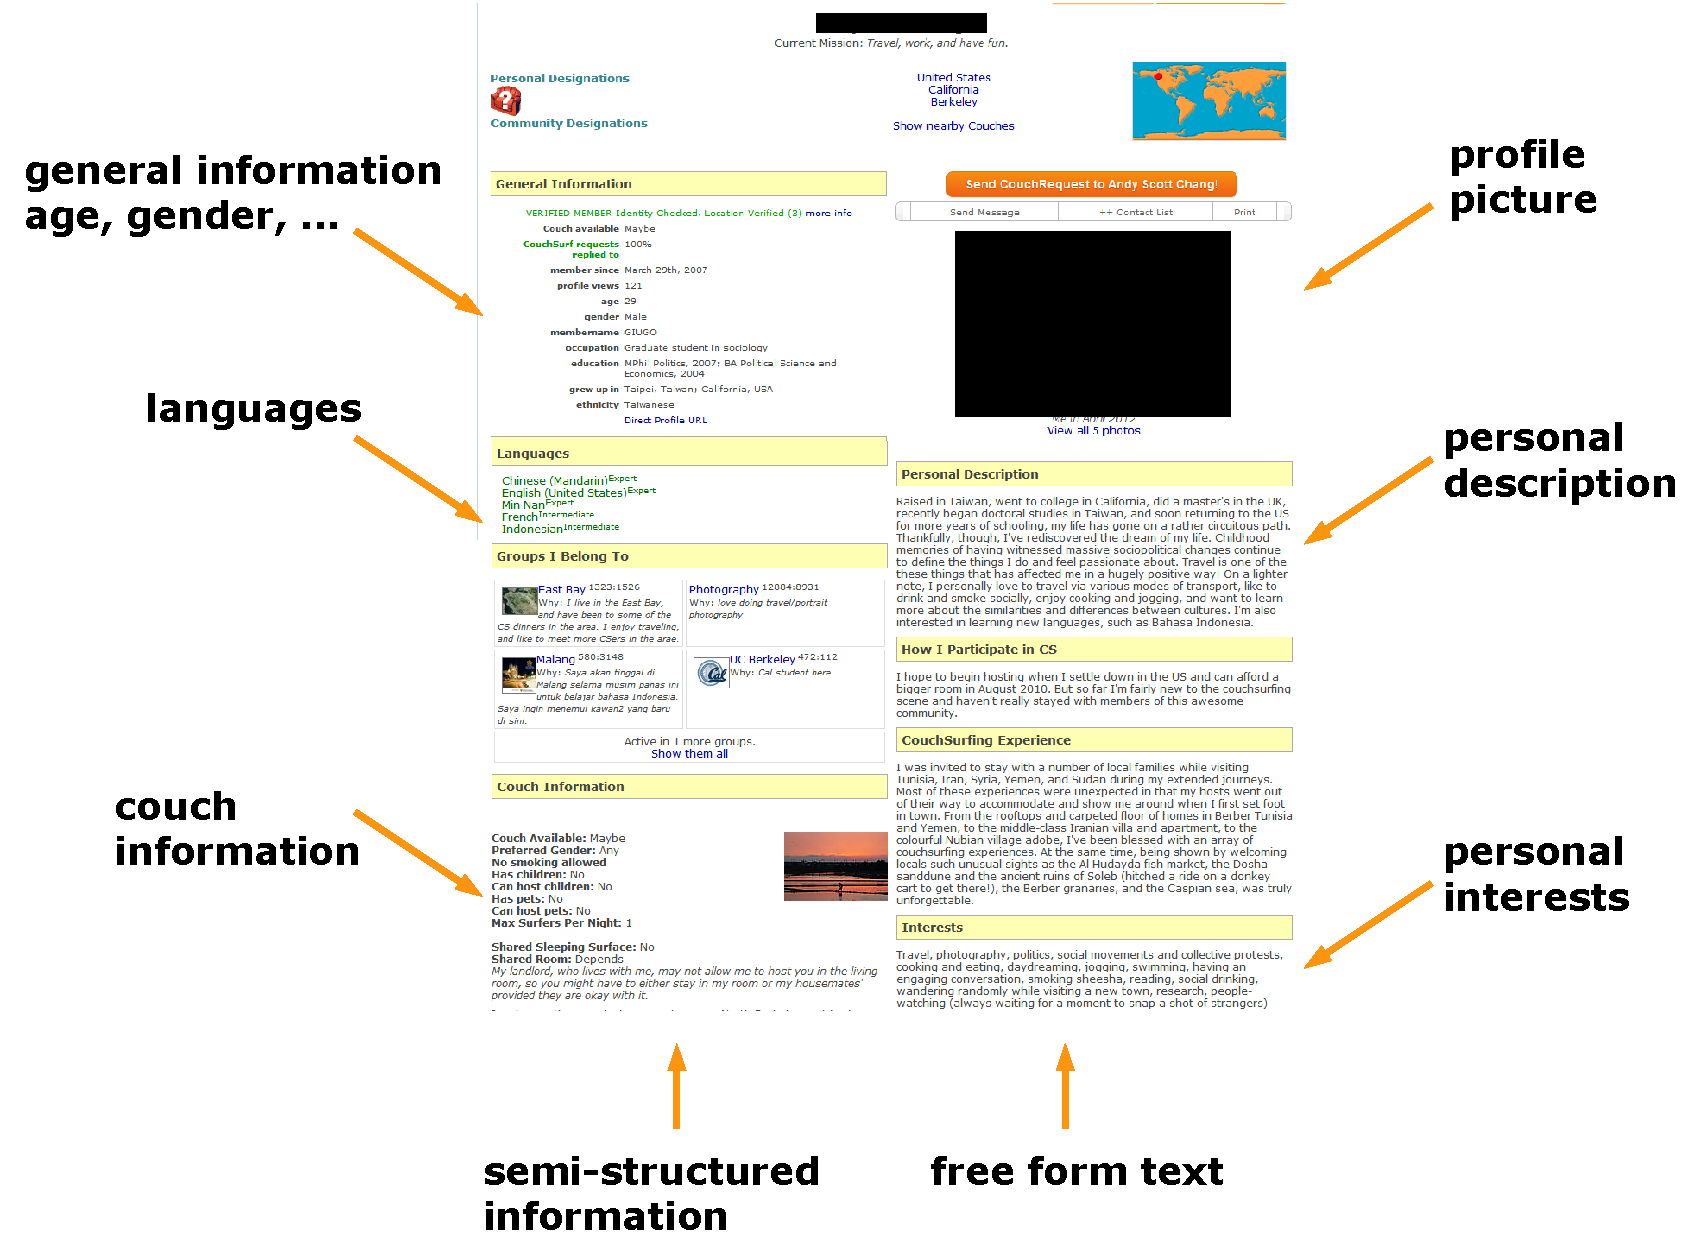
\includegraphics[width=1\linewidth]{./figures/csprofile.pdf}
\caption{User profiles on CouchSurfing.org contain lots of valuable information to estimate host and user preferences. While the left column is comprised of (semi-)structured information like age, gender, and languages spoken, whereas the right column solely consists of free textual descriptions.}
\label{fig:csprofile}
\end{figure}

With CouchSurfing becoming more popular it hasn't necessarily become easier to find a place to stay for surfers or find the right surfer to host. Potential hosts often get dozens of couch requests a day because the surfers need to send out more requests due to the increased competition between surfers. Particularly, hosts in popular locations are inundated with requests for accomodation (e.g. in New York City, Paris, London, Berlin, and Istanbul).

To achieve a good user experience, the acceptance rate of couchrequests needs to be high, i.e. the number of requests needed to eventually find a place should be minimized. On the other hand, hosts need assistance in deciding which surfer they would like to host. In this paper, we tackle both of these problems but focus on the latter (based on the expressed need of Developers at CouchSurfing). We estimate the probability that a user's couchrequest to a specific host is going to be successful based on the profiles of both user and host and the host's preferences. The couchrequests for a given host can then be re-ranked such that the best candidates are at the top (according to the hosts personal preferences). The couchsurfer benefits because we can show him the hosts that he is more likely to be accepted at minimizing his message-writing-efforts significantly. See Section \ref{sec:features} for a more detailed explanations which features we use to estimate this probability. The model for estimating it is described in Section \ref{sec:model}.
